\section{A First Pass at Quantum}
The early 1900's brought about a distinct revolution in our understanding of
physics. Certain issues in small-scale thermal physics were becoming more
apparent as the experiments and the theory became more precise.  The total
energy emitted by a black body radiator in the framework of classical theory was
infinite, while observations guaranteed that the average iron rod was not, in
fact, a source of infinite energy. Furthermore, the photoelectric effect, a
phenomenon in which a metal subjected to certain frequencies of light would emit
electrons, was not well-understood. It was thought at the time that these small
problems were the last remaining questions to be answered in physics, but they
would prove to be signs of a much greater misunderstanding of the physical
world.

Planck's solution to the black-body problem was intriguing. He achieved finite
predictions to black body energy radiation by assuming that the energy of the
radiation came in discrete quantized packets of energy, $E=h\nu$, where $h$ is
Planck's constant, and $\nu$ is the frequency of the light emitted. While Planck
used this method merely as a calculation tool, Einstein showed that
such an assumption has a more physical interpretation.

The problem with the photoelectric effect was as follows: the electrons that
eject from the metal have energy values that only depend on the \em
frequency\em, not the intensity, of the light impinging on them. Furthermore,
below a certain color frequency, no electrons would be emitted at all,
regardless of intensity. In the classical theory, light is modeled as a
continuous electromagnetic wave. In this model, the average power of a pure
EM wave is given as
\[
    P_{avg} = \frac{Af}{2}
\]
where $A$ is the amplitude, and $f$ is the frequency of the light. In this
model, any frequency of light--given a high enough amplitude--can deliver enough
energy to ionize the electrons in the metal. However, experiments showed that
this was not the case. Below a certain frequency, electrons would not be ionized
by the impinging light, regardless of intensity.

Einstein's solution to the problem was to assume that the energy delivered to
the metal was not continuously delivered--it came in discrete quantized packets
he called photons with energy $E = h\nu$. In this interpretation, the intensity
of light describes how many of these photons are emitted per second, and the
frequency of the light describes the amount of energy contained in a single
photon. The dynamics of the photoelectric effect are determined by the
interactions of the individual photons with the metal. This explains why the
frequency of light, not the intensity, dictated the energy of the electrons
emitted.

Both Planck's black body solution and Einstein's photoelectric solution hint at
a more complicated physical model than the classical theory described.
As it turns out, these complications are more than just changes in the form of
equations of motion: they require an entirely new mathematical system to
describe the theory.

For more information on the experimental development of quantum mechanics, see
\cite[p. 1-16]{Hall2013}.
%transition better?

\subsection{The Rules of Quantum Mechanics}

In this section, we will introduce the basic rules that describe the
mathematical system of quantum mechanics, as well as its connection to the
physical world.  To make things simple, only systems of a single particle will
be considered. Rules one and two describe the objects that make up the
theory, rules three and four describe how they behave to produce physical
results, and rule five describes how these objects evolve in
time.\cite[p. 64]{Hall2013}
\\
\\
\textbf{Rule 1}: The state of a quantum system is given by a unit vector
(usually denoted $\psi$) in some Hilbert space \textbf{H}. Furthermore, two
unit vectors $\psi_1$ and $\psi_2$ are equivalent (in the sense that they represent
the same physical state) iff $\psi_1 = c\psi_2$ for some $c \in \mathbb{C}$.

While the Hilbert space used will often change from system to system, it is
usually taken to be $L^2$ on some appropriate domain. In the simple case of a
particle moving in $\mathbb{R}^1$, for example, the Hilbert space associated
with such a system is $L^2(\mathbb{R})$.
Unit vectors in the Hilbert space are known as wavefunctions and multiplication
by a complex scalar is known as a phase shift.
\\
\\
\textbf{Rule 2}: For each function $f$ on the classical phase space there is
associated a self-adjoint operator $\hat{f}$ on the quantum Hilbert space
\textbf{H}. Such an operator is known as a quantum observable.

The process of obtaining $\hat{f}$ from $f$ is known as quantization. For the
most part, it is not necessary to consider quantizations of all possible phase
space functions, but only of a few key variables like position,
momentum, and energy. While there are known methods for quantization of
arbitrary functions, such methods are beyond the scope of current investigation
(see \cite[p.255-275]{Hall2013} for a more complete discussion of quantization
schemes).  The key quantization results are those for position and momentum. For
position, $\hat{x} = M_x$, the operator of multiplication by $x$. For momentum,
$\hat{p} = -i\hbar
\frac{d}{dx}$.

In most cases, the operator $\hat{f}$ will be unbounded. This arises from the
fact that the position and momentum operators, which will be explored in detail
in the next section, are themselves usually unbounded. For unbounded operators,
the notion of self-adjointness becomes a bit more complicated, but will be
explored in detail later on.
\\
\\
\textbf{Rule 3}: The probability distribution for the measurement of some
observable $\hat{f}$ for a quantum state $\psi$ satisfies
\[
    \langle f \rangle = \langle \psi, \hat{f}\psi \rangle
\]
where $\langle f \rangle$ is the expectation value of $f$.


Finding the probability distribution for an observable is the main objective of
a quantum mechanics problem, and is typically done with the linear algebra tools
of diagonalization, or spectral decomposition.

Consider a specific state $\psi_{\lambda}$ such that
$\hat{f}\psi_{\lambda} = \lambda \psi_{\lambda}$.
In this case, the expectation value of $f$ is given as
\[
    \begin{aligned}
        \langle f \rangle &= \langle \psi_{\lambda},
        \hat{f}\psi_{\lambda} \rangle\\
        &= \langle \psi_{\lambda}, \lambda \psi_{\lambda} \rangle\\
        &= \lambda \langle \psi_{\lambda}, \psi_{\lambda} \rangle\\
        &= \lambda.
    \end{aligned}
\]
As it turns out, the only probability distribution that satisfies these
conditions is the $\delta$ distribution at $\lambda$. In other words,
measurement of the variable $f$ on the state $\psi_{\lambda}$ will always
result in $\lambda$.

Ideally, one would find a complete set of such eigenstates. Then, each quantum
state in the system could be expressed as a linear combination of eigenstates 
$\psi = \sum_{n} c_n\psi_{\lambda_n}$.
The probability of measuring $\lambda_n$ for the variable $f$ would then be given as
$|c_n|^2$. While this assertion is not directly derivable from the previous
results \cite[p. 67]{Hall2013}, it is a very reasonable assumption to make. Since
$\psi$ is a unit vector, $\sum |c_n|^2 = 1$, and the expectation value for $f$
is readily seen to be consistent with this assumption.

Extending this method from the case of discrete eigenvalues to a continuous
spectrum is possible, and will be extensively explored later in this paper.
\\
\\
\textbf{Rule 4}: Suppose $\psi$ represents an initial state of a quantum system,
and suppose a state variable $f$ is measured to have a value $\lambda \in
\mathbb{R}$. Then, immediately following the measurement, the system will be in
a new state $\psi '$ satisfying
\[
    \hat{f}\psi ' = \lambda \psi '.
\]

The transition of the wavefunction from $\psi$ to $\psi '$ is known as the
collapse of the wavefunction. This rule makes intuitive sense: measuring a
variable twice in rapid succession should yield very similar, if not identical,
results. Collapse is frequently used to set up quantum mechanical systems. If
one desires a wavefunction in a particular eigenstate $\psi_{\lambda}$ of an
observable $f$, one could construct and ensemble of identical systems, and
measure $f$ on each system until the measurement yields $\lambda$ (for further
discussion of such a setup, see \cite{griffiths2005}). For observables
whose eigenstates are stationary in time, the wavefunction is then guaranteed to
stay in the state
$\psi_{\lambda}$.
\\
\\
\textbf{Rule 5}: The time evolution of a state $\psi$ is governed by the
Schrodinger equation:
\[
    \partial_t \psi = \frac{1}{i\hbar}\hat{H}\psi
\]
where $\hat{H}$ is the observable obtained from the classical Hamiltonian of the
system.

It is not difficult to see that this differential equation is solved with
\[
    \psi(t) = e^{\frac{-it\hat{H}}{\hbar}}\psi_0.
\]

(For an exploration of this \em operator valued exponential \em, see \cite[p.
74,208]{Hall2013}).
In the case that $\hat{H}$ has eigenfunctions
${e_n}$ and eigenvalues ${E_n}$ that form an orthonormal basis for \textbf{H},
the exponential becomes
\[
    e^{\frac{-it\hat{H}}{\hbar}}e_n = e^{\frac{-iE_nt}{\hbar}}e_n
\]
which extends linearly to arbitrary states
\[
    \begin{aligned}
        \psi &= \sum_n c_n e_n\\
        e^{\frac{-it\hat{H}}{\hbar}}\psi &= \sum_n c_n
        e^{\frac{-iE_nt}{\hbar}}e_n.
    \end{aligned}
\]

Of course, it is unreasonable to expect $\hat{H}$, which is only guaranteed to
be self-adjoint, to have an orthonormal basis of eigenfunctions. However, we
will see that the spectral theorem gives a way to generalize the notion of
eigenfunction such that we can define $e^{\frac{-it\hat{H}}{\hbar}}$ for any
Hamiltonian.

The eigenvalues of $\hat{H}$ hold special significance in quantum mechanics, as
they govern how the system evolves in time. Solving the Schrodinger equation, in
light of this result, usually boils down to solving the time-independent
Schrodinger equation
\[
    \hat{H}\psi=E\psi
\]
or more generally, finding the spectral decomposition of $\hat{H}$.


\subsection{An Example: The Infinite Square Well}

The most pertinent difference between classical physics and quantum physics lies
in the discretization of certain state variables of the system. To illustrate
this difference, consider the simple setup of a particle of mass $m$ in a
one-dimensional infinite square well potential
\[
    V(x) =
    \begin{cases}
        0 & \text{if } x\in[0,a]\\  \infty & \text{else}
    \end{cases}
\]
The relevant Hilbert space for this problem is $L^2(\mathbb{R})$, although the
wavefunctions for this problem will be required to be zero outside $[0,a]$.
The Hamiltonian for the system is the free particle Hamiltonian, given as
\[
    \hat{H} = -\frac{\hbar^2}{2m}\frac{d^2}{dx^2}
\]
inside the well.

The standard quantization of kinetic energy uses the identity
\[
    KE = \frac{p^2}{2m}
\]
which implies that
\[
    \widehat{KE} = \frac{-\hbar^2}{2m}\frac{d^2}{dx^2}
\]
Since the Hamiltonian is the sum of the kinetic and potential energy of the
particle, and the particle has no potential energy inside the well, it follows
that the Hamiltonian is as we stated.

Our goal is to decompose an arbitrary state into eigenstates of this
Hamiltonian. This will tell us the allowed energy values for the specified
potential. To do so, let's set up the time-independent Schrodinger equation
$\hat{H}\psi = E\psi$.
This leads to the equation
\[
    -\frac{\hbar^2}{2m}\frac{d^2}{dx^2}\psi = E \psi
\]

Solving this second order differential equation yields
\[
    \psi_E(x) =
    A\sin\left(\sqrt{\frac{2mE}{\hbar^2}}x\right) +
    B\cos\left(\sqrt{\frac{2mE}{\hbar^2}}x\right).
\]

Now, we can impose boundary conditions. By requiring that the wavefunction be
zero at the ends of the well when the potential is infinite, the following
conclusions can be made:
\begin{center}
\begin{tabular}{l l}
    $\psi(0) = 0 \implies$  & $B = 0$\\
    $\psi(a) = 0 \implies$  & $E = \frac{n^2\pi^2\hbar^2}{2ma^2}$
\end{tabular}
\end{center}

The condition on $E$ gives us a characterization of the spectrum of $\hat{H}$.

Furthermore, the wavefunction is required to have unit length. This means
\[\langle \psi, \psi \rangle = 1\]
or
\[\int_{[0,a]} A\sin\left(\sqrt{\frac{2mE}{\hbar^2}}x\right)
          \overline{A\sin\left(\sqrt{\frac{2mE}{\hbar^2}}x\right)}dx = 1\]

which restricts $A$ to the value of $\sqrt{\frac{2}{a}}$.

Thus, we have a complete characterization of the eigenstates of the Hamiltonian:
\[
    \psi_E(x) = \sqrt{\frac{2}{a}}\sin\left(\frac{n\pi}{a}x\right).
\]

It is a standard result (\cite[p. 89]{Folland2009})
that such functions are dense in the solution space
$L^2([0,a]) \subset L^2(\mathbb{R})$. So any wavefunction $\psi(x)$ can be written
as
\[
    \psi(x) =
    \sum_{n=1}^{\infty} c_n \sqrt{\frac{2}{a}}\sin\left(\frac{n\pi}{a}x\right)
\]
with coefficients given by
\[
    c_n = \int_{[0,a]} \psi(x)\sqrt{\frac{2}{a}}\sin\left(\frac{n\pi}{a}x\right)dx
\]
Furthermore, given an initial state $\Psi(x,0) = \psi(x)$, the full
time-evolution solution to this potential is
\[
    \Psi(x,t) =
    \sum_{n=1}^{\infty} c_n
    e^{\frac{-iE_nt}{\hbar}}\sqrt{\frac{2}{a}}\sin\left(\frac{n\pi}{a}x\right)
\]
with $E_n = \frac{n^2\pi^2\hbar^2}{2ma^2}$ for $n\in \mathbb{N}$.

Classically, one could imagine a particle in a box with any arbitrary kinetic
energy. However, in quantum this is not the case. Notice how the allowed energy
states are quantized: values like $E = \frac{17\pi^2\hbar^2}{2ma^2}$ do not show
up in the spectrum of $\hat{H}$, so they will not be measured. The particle
cannot have any arbitrary definite energy.

\subsection{The Finite Square Well: Continuous vs Discrete Spectra}

Consider a similar potential function, the finite square well
\[
    V(x) =
    \begin{cases}
        -V_0 & \text{if } x\in[-a,a]\\
        0 & \text{else}
    \end{cases}
\]
for some positive potential height $V_0$.

This time, the Hamiltonian is piecewise defined as
\[
    \hat{H}(x) =
    \begin{cases}
        \frac{-\hbar^2}{2m}\frac{d^2}{dx^2} - V_0& \text{if } x\in[-a,a]\\
        \frac{-\hbar^2}{2m}\frac{d^2}{dx^2} &\text{else}
    \end{cases}
\]
which will operate on the Hilbert space $L^2(\mathbb{R})$.

Again, our goal is to find the eigenfunctions (or a more general spectral
decomposition) of this Hamiltonian on $L^2(\mathbb{R})$.
The complicating factor here is the fact that the Hamiltonian is actually
unbounded on $L^2(\mathbb{R})$. For example, there are many functions in
$L^2(\mathbb{R})$ that do not have square-integrable second derivatives, so
$\hat{H}$ cannot act on them. Therefore, it is
necessary to impose stricter conditions on our solutions. Namely, $\psi$ is
required to be continuous with a continuous first derivative. Note that $\psi$
may not have a defined second derivative at the points of discontinuity $x=a,
x=-a$, but since this is a set of measure zero, the second derivative can still
be computed in $L^2$ space.

If we assume $E<0$, we find that
\[
    \psi(x) =
    \begin{cases}
        C_1e^{\sqrt{\epsilon}x}& \text{if } x\in(-\infty,-a]\\
        C_2\cos(\sqrt{v-\epsilon})& \text{if } x\in[-a,a]\\
        C_3e^{-\sqrt{\epsilon}x}& \text{if } x\in [a, \infty)
    \end{cases}
\]
Where $\epsilon = -\frac{2mE}{\hbar^2}$ and
$v=\frac{2mV_0}{\hbar^2}$.

Applying the continuity conditions necessary for $\psi$ to be in the domain of
the Hamiltonian and applying some basic algebra, we find that
\[
    \sqrt{\epsilon} = \sqrt{v-\epsilon}\tan(\sqrt{v-\epsilon}a)
\]
This equation is transcendental, so there are no closed-form solutions to
$\epsilon$, but the existence of solutions can be seen by graphing
$\sqrt{\epsilon}$ and $\sqrt{v-\epsilon}\tan(\sqrt{v-\epsilon}a)$ (see \cite[p.
78-80]{griffiths2005}).
However, there are only finitely many $\epsilon$ for which this is true. That
is, there are only finitely many energy states that are "bound" to the
potential.

\begin{figure}
    \begin{center}
    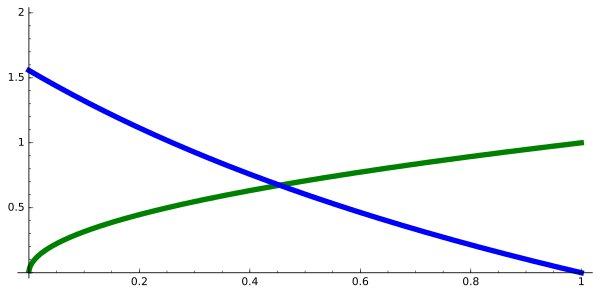
\includegraphics[scale=0.5]{transcendental_solutions}
    \caption{A plot of the functions $f(x) = \sqrt{x}$ and
    $g(x)=\sqrt{1-x}\tan(\sqrt{1-x})$. Their intersection point marks a solution
        to the transcendental equation $\sqrt{x} = \sqrt{1-x}\tan(\sqrt{1-x})$.}
    \end{center}
\end{figure}

What if we restrict attention instead to the case $E>0$? Applying a similar
analysis to what was done in the infinite square well case, the solutions can be
found to be linear combinations of complex exponentials. There is no inherent
restriction on the energies allowed in this case, since there are no boundary
conditions to match. However, a single complex exponential $\psi(x) = e^{ikx}$
is not in $L^2(\mathbb{R})$, since the integral
$\int_{\mathbb{R}}e^{ikx}\overline{e^{ikx}}dx$
diverges to infinity, and thus is not in the domain of the Hamiltonian.

While a single complex exponential may not be square-integrable, an infinite sum
of them might be. Using some elementary results from Fourier analysis(see
\cite[Thm. 8.4.1]{Lang1993}), it can be
shown that the function
\[
    \psi(x) = \int_{\mathbb{R}} \phi(k)e^{ikx}dx
\]
is square-integrable for $\phi$ a Schwartz function (a function that rapidly
decays to zero).

In this sense, the state $e^{ikx}$ is a sort of "pseudo-eigenstate". By itself,
the state is not in $L^2(\mathbb{R})$, but a continuous sum of these states,
which physicists refer to as a "wave packet", can
be in $L^2(\mathbb{R})$. This concept will be made much more complete with the
tools of the spectral theorem.

For a more detailed derivation of these results, see \cite[p. 109-120]{Hall2013}
and \cite[p. 78-82]{griffiths2005}.
